\documentclass[a4paper,11pt]{article}
\usepackage[utf8]{inputenc}

% extra packages
% \usepackage{amsrefs}
% \usepackage[autocite=inline,labelalpha=true]{biblatex}

%\usepackage[top=1in, left=1in, right=1in, bottom=1in]{geometry}
\usepackage[top=1.2in, left=1.2in, right=1.2in, bottom=1.5in]{geometry}
\usepackage{wrapfig}
\usepackage{amsmath, amssymb}
\usepackage{graphicx}
\usepackage{color}
\usepackage{hyperref}
\usepackage{siunitx}

\DeclareUnicodeCharacter{03F5}{\ensuremath{\epsilon}}

\newcommand{\pa}{\partial}
\newcommand{\ve}{\varepsilon}
\newcommand{\h}{\mathcal{H}}

%\setlength{\parindent}{0pt}

\begin{document}
	
	\begin{center}
		\Large \textbf{Research Statement}
		
		\Large Youngmin Park
	\end{center}
	
	\begin{itemize}
		\item \textbf{Mathematical themes}: Stochastic and deterministic dynamical systems. Oscillators, separation of timescales, bifurcation theory, master equation.
		\item\textbf{Biological themes}: Biological neural networks. Cortical function, molecular motor transport, gene expression.
	\end{itemize}
	
	\section{Research Overview}
	
	I develop dimension-reduction methods for neural network models using stochastic and deterministic \textbf{dynamical systems theory}. In turn, I use these methods to understand the function and maintenance of biological and chemical networks within the context of \textbf{neuroscience}. My work is highly \textbf{interdisciplinary with excellent funding potential}. My publication record demonstrates my ability to produce high-impact work with researchers of diverse backgrounds, including neuroscientists \cite{park2020circuit,shaw2012phase}, engineers \cite{ermentrout2019recent,park2021high}, mathematical neuroscientists \cite{park2016weakly,park2018infinitesimal,park2018multiple,park2018scalar}, and fluid dynamicists \cite{park2020dynamics,park2021coarse,fai2020global}. My research program includes the following sub-directions:
	
	\begin{itemize}
		\item \textbf{Neural Oscillators, Section \ref{sec:interactions}}. I introduce generalizations of weakly coupled oscillator theory to strong coupling. This work enables engineers to design optimally controlled systems related to rhythms such as heart beats, sleep cycles, and central pattern generators.
		\item \textbf{Neural Maintenance, Section \ref{sec:maintenance}}. I analyze the dynamics of molecular motors, which are necessary for cell function in all animals. Research includes developing a master equation of motor states coupled to a PDE describing the underlying motor positions and the exploration of discrepancies in stochastic and deterministic models related to Keizer's paradox.
		\item \textbf{Undergraduate Research, Section \ref{sec:undergrad}}. My work is accessible to a broad spectrum of skills and backgrounds in STEM (although I strongly encourage students from other backgrounds to participate in my research). My goal is to equip students with programming and scientific literacy skills, which they can use to enhance their lives and careers.
	\end{itemize}
	%I conclude with a comprehensive research plan in Section \ref{sec:research}.
	
	\section{Neural oscillators}\label{sec:interactions}
	
	%The mammalian neocortex is a key region for numerous functions such as sensory perception and integration, generation of fine motor commands, spatial reasoning, and human language \cite{fuster2002frontal}. Over the past century, researchers have established that the neuron is the computational unit of the cortex, and dense networks of neurons ultimately give rise to complex thought. However, the sheer number and density of connections per cubic spatial unit of cortex poses a daunting scientific challenge. Dimension reduction techniques are invaluable to aid in this endeavor.
	
	%\subsection{Previous Work}
	
	%\textbf{How does the cortex produce patterned activity?} Spatially-modulated neurons such as head direction, place, and grid cells, produce spatio-temporal brain activity that is fundamental to spatial memory and animal survival. The mechanisms underling this activity are not yet well-understood and are difficult to understand from a mathematical and neurobiological perspective. I introduced a method to reduce the dimension of large neural networks, allowing an exploration of the underlying neural mechanisms in great detail. I discovered that interactions between neural adaptation and external inputs contribute to the complex motion of patterned activity in the cortex \cite{park2018scalar}. Only a small set of simple mechanisms can lead to substantial changes in the brain.
	
	%\textbf{How does the cortex control brain rhythms?} In addition to spatio-temporal activity, cortical rhythms are ubiquitous and implicated in behavioral tasks such as attention, memory, and motor coordination. Moreover, large cortical networks produce rhythms that are subject to ever-changing concentrations of neuromodulators. The mechanism of how neuromodulators alter rhythms, and therefore attention, is not well-understood. To better understand this mechanism, I introduced a theory to understand acetylcholine's role in changing the synchronization properties of cortical oscillators. My theory showed that neuromodulators alter the phase response curve (PRC) of neurons and therefore alter the large-scale brain rhythms \cite{park2016weakly}. I extended this result to include strongly asynchronous populations of neurons \cite{park2018multiple}, facilitating future studies of more realistic networks of heterogeneous neurons.
	
	%\textbf{How does the brain process sounds?} The auditory cortex processes sounds in simple but important ways. For example, the auditory cortex adapts to constant background noise by responding less strongly over time, but will respond strongly to sudden changes in the auditory environment. This function is critical to the survival of many animals. To understand how auditory signals are processed, numerous optogenetics labs established differential roles of inhibitory neuron subtypes in processing auditory signals. Labs used different experimental paradigms, so the fundamental role played by each inhibitory subtype was unclear. I unified the experimental results using a single cortical model. The model suggests that numerous brain functions can derive from relatively simple circuits \cite{park2020circuit}.
	
	%
	%\begin{itemize}
	% \item \textbf{Park, Y.} and Geffen, M.N. \textit{A Mechanistic Model of the Auditory Cortex with Inhibitory Subtypes} (in preparation). We introduce a groundbreaking model of cortical responses to complex auditory stimuli, which includes inhibitory subtypes implicated in such auditory processing. The model readily generates hypotheses for the role of these inhibitory subtypes across multiple experimental results.
	%
	% \item \textbf{Park, Y.}, Shaw, K.M. Chiel, H.J. Thomas, P.J. \textit{The Infinitesimal Phase Response Curve of Oscillators in Piecewise Smooth Dynamical Systems}. European Journal of Applied Mathematics (2018). We provide a first-principles derivation of the phase response curves (PRCs) of oscillators satisfying non-smooth dynamics. This work is a much-needed extension of the half-century-old theory of PRCs.
	% 
	% \item \textbf{Park, Y.}, Ermentrout, G.B. \textit{Weakly Coupled Oscillators in a Slowly Varying World}. (2016). We extend the theory of weakly coupled oscillators to account for a slowly varying parameter, greatly facilitating more realistic and topical studies using dynamic parameters. 
	%  
	% \item \textbf{Park, Y.}, Ermentrout, G.B. \textit{Scalar Reduction of a Neural Field Model with Spike Frequency Adaptation}.
	% SIAM Journal on Applied Dynamical Systems (2018). We introduce a novel dimension reduction of so-called ``bump'' solutions of non-local neural field models to centroid coordinates. The dimension reduction allows for a comprehensive analysis of the many bifurcations of the system with greater generality than previously possible.
	% 
	% \item \textbf{Park, Y.}, Ermentrout, G.B. \textit{A Multiple Timescales Approach to Bridging Spiking- and Population-level Dynamics}. (2018). We introduce a powerful theory that robustly accounts for large frequency differences between populations. This substantial contribution enables computational works to operate without the classic restraint of small frequency differences.
	% 
	% \item \textbf{Park, Y.}, Heitmann, S., Ermentrout, G.B. \textit{The Utility of Phase Models in Studying Neural Synchronization}. Book chapter in Computational Models of Brain and Behavior. Wiley-Blackwell (2017). In this book chapter, we explore how different types of phase response curves and synaptic connections affect the synchronization properties of a network. This chapter is the first to address this relationship directly, and provides a much-needed guideline for future computational studies.
	% 
	% \item Shaw, K.M., \textbf{Park, Y.}, Chiel, H.J., Thomas, P.J. \textit{Phase Resetting in an Asymptotically Phaseless System}. SIAM Journal on Applied Dynamical Systems (2012). We derive explicit equations for the phase response curve of a planar, piecewise-linear dynamical system. In contrast to existing beliefs, the work proves that transitions between boundaries can have the greatest effect on the phase response curve.
	%
	%\end{itemize}
	%\subsection{Ongoing Work}
	
	%\cite{ott2008low,kopell2014beyond,nicks2018clusters}
	%\cite{golubitsky1986hopf,golubitsky2003symmetry,murza2011oscillation}
	%\cite{coombes2001phase,ermentrout2002modeling,coombes2012nonsmooth}
	
	My work on oscillations falls within broader goals oriented towards understanding pathological neural behavior such as Parkinsonian tremors, epilepsy, and cardiac alternans. Overall theoretical work in these directions has been promising but tends to use one of three starting points: mathematically tractable but very abstract models, particular forms of symmetry, and the \textit{weak coupling} assumption (or more generally, the \textit{linear} approximation) \cite{ermentrout2002modeling}. The weak coupling assumption has long been an invaluable theoretical tool to understand neural behavior consisting of only small deviations from a known state such as quiescence or oscillatory activity. Indeed, the weak coupling assumption has driven much of my work \cite{park2016weakly,park2018multiple,park2018scalar}. 
	
	While these assumptions continue to facilitate theorists to a potent degree, they are now far from modern experimental conditions, which are often performed \textit{in vivo}. In this environment, neurons are often strongly coupled, heterogeneous, and interact nonlinearly. These properties persist in both healthy and pathological neural function, so it follows that pathologies can not always be understood using abstraction, symmetry, or linearity. Therefore, my field must develop theories that directly address \textit{strongly coupled} networks of \textit{heterogeneous} neurons with \textit{nonlinear} interactions at multiple scales. We must understand the brain as it is.
	
	To this end, \textit{I have formulated a theory of strongly coupled oscillators} \cite{park2021high}. Consider the coupled system of $N$ ODEs,
	\begin{equation}\label{eq:odes}
		\dot X_i = F(X_i) +\ve \sum_{j=1}^N a_{ij} G(X_i,X_j), \quad i=1,\ldots,N,\\
	\end{equation}
	where each system admits a $T$-periodic limit cycle $Y(t)$ when $\ve=0$. We allow $\ve>0$ not necessarily small and assume general smooth vector fields $F:\mathbb{R}^n \rightarrow \mathbb{R}^n$ and a smooth coupling function $G:\mathbb{R}^n\times\mathbb{R}^n\rightarrow \mathbb{R}^n$. The scalars $a_{ij}$ modulate coupling strength between pairs of oscillators, whereas $\ve$ modulates the network's overall coupling strength.
	
	Let $\theta_i$ be the phase of limit cycle $Y_i$ and define the phase difference $\phi_i=\theta_i-\theta_1$ for $i=2,\ldots,N$. Under general conditions, it is possible to derive a phase reduction of $N-1$ equations,
	\begin{align*}
		\dot \phi_i =& \ve\sum_{j=1}^N a_{ij} \h(-\phi_i,\phi_2-\phi_i,\ldots,\phi_N-\phi_i,\phi_j-\phi_i)\\
		&\quad- \ve\sum_{j=1}^N a_{ij} \h(0,\phi_2,\ldots,\phi_N,\phi_j), \quad i=2,\ldots,N,
	\end{align*}
	where
	\begin{equation*}
		\h(\eta_1,\ldots,\eta_N,\xi) = \frac{1}{T} \int_0^T \mathcal{Z}(\eta_1+s,\ldots,\eta_N+s) \cdot G(s,\xi+s)ds,
	\end{equation*}
	and $\mathcal{Z}$ is the higher-order phase response curve from \cite{wilson2020phase}. My theory produces Taylor truncations of the function $\h$ in powers of $\ve$. The higher the truncated order, the more accurately my theory reproduces phase-locked states of $N$ oscillators.
	
%	\begin{figure}[ht!]
%		\centering
%		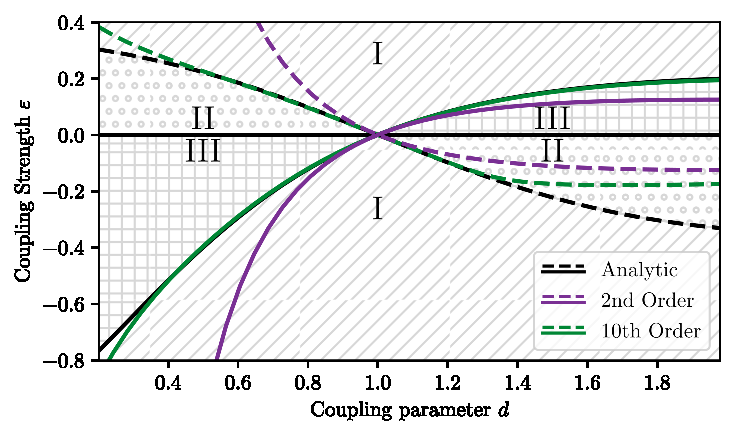
\includegraphics[width=.75\textwidth]{figures/cgl_2par_edited.pdf}
%		\caption{Validation of strong coupling theory using diffusively coupled complex Ginzburg-Landau (CGL) models. The plot is a two-parameter bifurcation diagram in coupling parameters $\ve$ and $d$. Synchrony is only stable in regions I and II, whereas antiphase is only stable in regions I and III. Black solid lines denote boundaries where the system switches between stable and unstable synchrony ($\ve_s$). Black dashed lines denote boundaries where the system switches between stable and unstable antiphase ($\ve_a$). Purple solid, dashed: bifurcations detected using second-order interaction functions from \cite{wilson2019phase}. Green solid, dashed: bifurcations detected using tenth-order interaction functions. \textbf{This result shows that my strong coupling theory substantially outperforms existing coupling theory.}}\label{fig:cgl}
%	\end{figure}
	
	I tested my theory using a realistic four-dimensional model of a thalamic neuron. Figure \ref{fig:thal} shows how my theory predicts phase differences in two thalamic oscillators for different coupling strengths (higher order corresponds to greater accuracy). The right-hand side of the reduced phase-difference ODE (labeled $-2\h_{\text{odd}}$) is shown in the top row. Roots and slopes correspond to the existence and stability of phase-locked states. Phase differences of the full model are shown in the bottom row for 20 different initial conditions. Coupling strength increases from weak ($g_\text{syn}=0.02$, left column) to strong ($g_\text{syn}=0.25$, right column). \textbf{Roots of the fourth-order reduction coincide with the steady-state phase-locked states of the full system}.
	
	\begin{figure}[ht!]
		\centering
		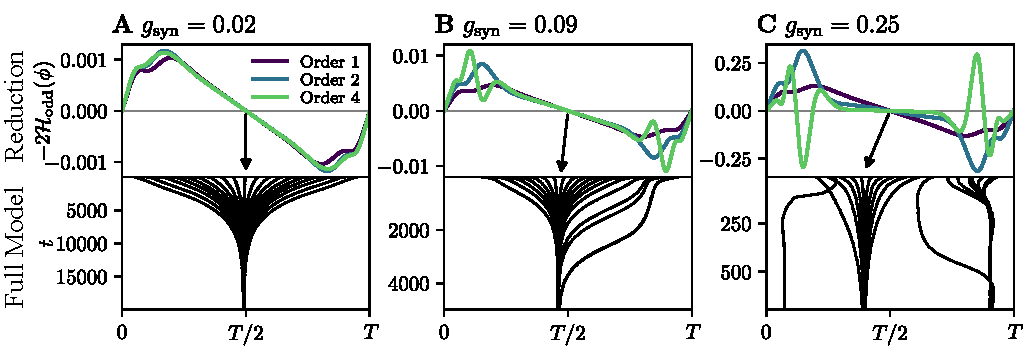
\includegraphics[width=\textwidth]{figures/thal_h_edited.pdf}
		\caption{Performance of the strong coupling reduction compared to a full simulation of thalamic neuron models. A: Weak coupling. The right-hand side of the reduction (top) is shown for different orders (higher orders correspond to greater accuracy) and coincides with the long-term phase difference of the full model (bottom). B: Moderate coupling. The reduction (top) coincides with the full model (bottom). C: Strong coupling. The reduction (top) only agrees with the full model (bottom) at order 4. }\label{fig:thal}
	\end{figure}
	
	\subsection{Future Work}
	I will further develop my method in several important directions. I will augment my theory to include heterogeneity (including n:m phase-locking), making my theory applicable to far more realistic neural networks. I will augment my theory to include oscillator death to understand interactions between bursting neurons in networks such as subcortical networks and central pattern generators. Finally, I will derive the mean-field equations for neural models (in contrast to existing mean-field theories that use idealized models) to understand how microscopic neural interactions influence large-scale brain activity.
	
	%This theory is well-suited to problems beyond neuroscience. For example, I have started a collaboration with the Fraden lab at Brandeis University, where I am applying strong coupling theory to problems of oscillatory reactions in star networks. Using this reduced model, I will uncover the mechanisms behind transitions in phase-locked patterns and account for the heterogeneity inherent in experimental reactions.
	
	\section{Neural Maintenance} \label{sec:maintenance}
	
	%\cite{kasai2010structural,holtmaat2009experience}
	Pyramidal neurons are the most ubiquitous type of neurons in the mammalian neocortex. They feature tens of thousands of excitatory convergent synaptic inputs, where most incoming synaptic signals terminate on sub-micron bulbs known as dendritic spines. Spines exhibit a significant degree of morphological plasticity, with pathological spine formation implicated in disorders such as Autism spectrum disorder and Alzheimer's disease \cite{penzes2011dendritic}. Therefore, how spines function and how they are maintained is an important question.
	
	%\cite{park2006plasticity,wang2008myosin}
	Dendritic spines receive surface proteins by protein-carrying vesicles that squeeze through spine neck and eventually fuse with the spine head. The motion of such vesicles has been observed to involve translocation, where the motion is unidirectional, corking, where the vesicle gets stuck in the spine neck, and rejection, where the vesicle initially enters the spine but eventually reverses direction and exits \cite{park2006plasticity}. \textbf{How molecular motors affect changes in vesicle direction is the goal of ongoing work}.
	
	%\cite{muller2008tug,kunwar2011mechanical}
	%\cite{bressloff2009directed,newby2009directed,newby2010random,newby2011asymptotic,bressloff2013metastability}
	%\cite{julicher1995cooperative,guerin2011motion,allard2019bidirectional,portet2019deciphering}
	However, existing studies often neglect or fix drag forces that could arise from constriction effects in the unique bulbous shape of dendritic spines. While I have recently published work relating dendritic morphologies to bidirectional motion \cite{park2020dynamics}, this work relies on mean-field equations and only established the existence and stability of velocities; it does not consider noise-dependent quantities such as the probability for vesicle to translocate or the mean first passage time (MFPT) to translocation.
	
	\begin{figure}[ht!]
		\centering
		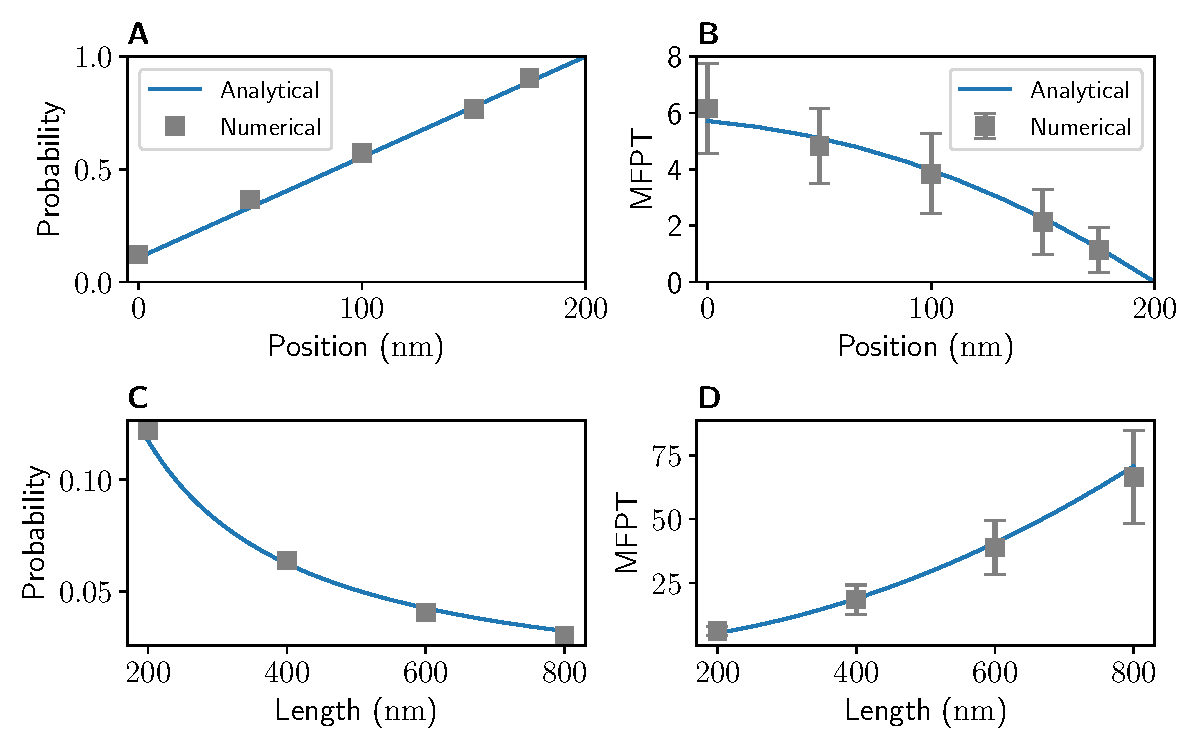
\includegraphics[width=\textwidth]{figures/f_mfpt_translocation.pdf}
		\caption{Probability and MFPT of translocation. A, B: Probability and MFPT of translocation as a function of initial vesicle position. C, D: Probability and MFPT of translocation as a function of spine length. MFPTs have dimensions of seconds.}\label{fig:mfpt}
	\end{figure}
	
	The formulation I consider includes two identical species that prefer to push the vesicle in opposite ``up'' and ``down'' directions. I coarse-grain a detailed agent-based model of the molecular motor and vesicle dynamics using a master equation formulation,
	\begin{equation*}
		\begin{split}
			\frac{\pa P_{ij}}{dt} &= -\left[\gamma_i(V) + \gamma_j(-V) + \alpha (N - i) + \alpha( N - j)\right]P_{ij}\\
			&\quad + \alpha(N - (i-1)) P_{i-1,j} + \alpha (N - (j-1)) P_{i,j-1}\\
			&\quad + \gamma_{i+1}(V)P_{i+1,j} + \gamma_{j+1}(-V)P_{i,j+1},
		\end{split}
	\end{equation*}
	where $P_{i,j}(t)$ is the probability of having $i$ up motors and $j$ down motors attached to the vesicle at time $t$, $\alpha$ is the attachment rate, $N$ denotes the total number of available motors for each species, and $\gamma_k(V)$ represents the velocity-dependent detachment rate. The velocity $V$ depends on the total force output of the motors, which depends on the distribution of motor positions described by an advection-reaction equation for each species,
	\begin{equation}\label{eq:advection}
		\frac{\pa}{\pa t}\phi\left(z,t\right) + V\frac{\pa}{\pa z}\phi\left(z,t\right) = -\beta \phi(z,t) + \alpha(1-\theta)\delta(z-A),
	\end{equation}
	where $\phi(z,t)$ denotes the motor position probability density, $z$ is the local motor position, $t$ is time, and $\theta$ is the proportion of attached motors. The delta function represents the position where molecular motors initially attach. The velocity is then $V \propto -\sum_i k x_i  + \sum_j k y_i$, where $x_i$ and $y_i$ are the positions of up and down motor species drawn from the distribution \eqref{eq:advection} at each time $t$ and $k$ is a spring constant. Further details on the efficiency improvements of the master equation, the distribution of waiting times, and numerical convergence are contained in my recent preprint \cite{park2021coarse}.
	
	Due to the constant-diameter constriction, the system can be well-approximated by a telegraph process. Plots of the numerical calculations from the master equation are shown in Figure \ref{fig:mfpt} as gray squares. The analytical calculations from approximating the master equation as a telegraph process are shown as blue lines.
	
	\subsection{Future Work}
	This work raises general questions about spine morphologies and control. Based on Figure \ref{fig:mfpt}, even moderately long dendritic spines on the order of \SI{600}{\nm} have a low probability of translocation. If the spine is made wider, the probability to translocate becomes greater. In contrast, especially thin spines tend to force unidirectional movement (data not shown). In future work, I will explore the broader impacts of these properties on neural function. %For example, how does the post-synaptic density correlate to spine morphology for a given neuron? Do neurons with majority long, thin spines tend to have more concentrated post-synaptic densities? If so, are such neurons involved in long-term storage of memories, or short term storage? Do neurons with majority short, stubby spines imply more synaptic plasticity? By addressing these questions, I will bridge the gap between dendritic physiology and neural function.
	
	In recent conversations with my current postdoctoral advisor St\'{e}phanie Portet, it was revealed that noise can stabilize molecular motor transport. They have run numerical calculations comparing deterministic and stochastic simulations. However, an analytical treatment remains to be performed. To determine how noise stabilizes motor transport, I will consider a simplified version of the model and establish the existence and stability of stationary distributions.
	
	\section{Undergraduate Research}\label{sec:undergrad}
	
	Studying biology through the lens of dynamical systems is an ideal framework to involve a diverse group of undergraduates in research. Problems I pursue are accessible to students from any STEM field who have an elementary understanding of calculus and ordinary differential equations. Such students can bring their unique perspectives from math, biology, ecology, chemistry, physics, or computer science to contribute to modeling biological phenomena. The principles they learn from formalizing a problem within a mathematical framework will teach them to extract essential characteristics of a system in order to generalize other properties. This method of thinking will serve them well throughout their undergraduate education and further into their careers.
	
	%My students will first learn the fundamentals of the field of their choosing. For example, a student interested in coupled oscillator theory will learn about phase response curves, return maps, and weak coupling theory. A student interested in molecular motor dynamics and cellular transport will learn about stochastic calculus, PDEs, and numerical analysis. I will introduce them to state-of-the-art research through journal club discussions. This process will lead them towards research questions of their choosing, and I will guide them towards tractable problems. Driven students will have opportunities to publish first-author papers in reputable journals and changes to share their work at conferences.
	
	Below are potential project ideas from simple to complex, to be given depending on the skill, interest, and commitment-time of the student. I remark that I fully understand the potential for a relatively unskilled and uninterested student to become a skilled and dedicated researcher, so this list is by no means a hard rule.
	
	\begin{itemize}
		\item (Simple) Reproduce figures from a paper of the student's choosing and present the main results. Generate potential research ideas based on the paper.
		\item (Simple) Help improve the documentation for my open source projects in coupled oscillators and molecular motor dynamics. Contribute features to these projects.
		\item (Moderate) Join an ongoing research project. For example, generate figures for a paper using a language and numerical integrator of their choosing. The student will be tasked with visualizing a particular problem and will be responsible for writing and debugging their code from top to bottom.
		\item (Complex) Lead a research project. For example, study the effects of splay states using strong oscillator coupling theory. Determine different types of bifurcations as a network transitions from different phase-locked states as a function of a network parameter, such as coupling strength.
	\end{itemize}
	
	
	\bibliographystyle{plain}
	\bibliography{refs.bib,../youngmin-bard/bio,../youngmin-bard/neuralfield,../youngmin-bard/math,../youngmin-bard/phase,../youngmin-bard/computation,../youngmin-bard/cortex,../thomas-youngmin/notes/spines.bib,../thomas-youngmin/notes/vesicles.bib,../thomas-youngmin/notes/noise.bib,../thomas-youngmin/notes/motors.bib}
	
	
\end{document}
